\documentclass[12pt,a4paper]{article}
\usepackage[table]{xcolor}
\usepackage{float}
\usepackage[spanish]{babel}
\usepackage{amsmath}
\usepackage{amssymb}
\usepackage{graphicx}
\usepackage{amsfonts}
\usepackage[utf8]{inputenx}
%\usepackage{algorithm2e}
\usepackage{listings}
\usepackage{pdfpages}
\usepackage{tabularx}
\usepackage{color}
\usepackage{anysize}
\usepackage{fancyhdr}
\usepackage{ulem}
%\usepackage{caption}
\usepackage[font=footnotesize]{caption}
\definecolor{deepblue}{RGB}{0,0,153}
\definecolor{deepred}{RGB}{153,0,0}
\definecolor{deepgreen}{RGB}{51,102,0}
\definecolor{deepyellow}{RGB}{204,204,0}
\marginsize{2cm}{2cm}{1cm}{1.5cm} % depende de anysize
%\renewcommand*{\thefootnote}{\Roman{footnote}}
\lstset{ %
			language=Python,
			basicstyle=\footnotesize,
			numbers=left,
			stepnumber=1,
			numbersep=4pt,
			tabsize=2,
			otherkeywords={self}, 
			keywordstyle=\color{deepred},
			stringstyle=\color{deepgreen},
			commentstyle=\color{deepblue},
}
\usepackage{hyperref}
\hypersetup{
    colorlinks=true,
    citecolor=black,
    filecolor=black,
    linkcolor=black,
    urlcolor=black,
    linktoc=all
}



%\title{Multímetros en Corriente Continua}
\title{TP Final}
\author{
        Grupo 1
}
\date{\today}
\pagestyle{fancy}
\lhead{Facultad de Ingenieria}
\rhead{Laboratorio - 66.02 - Curso 001 - TP Final}


\begin{document}
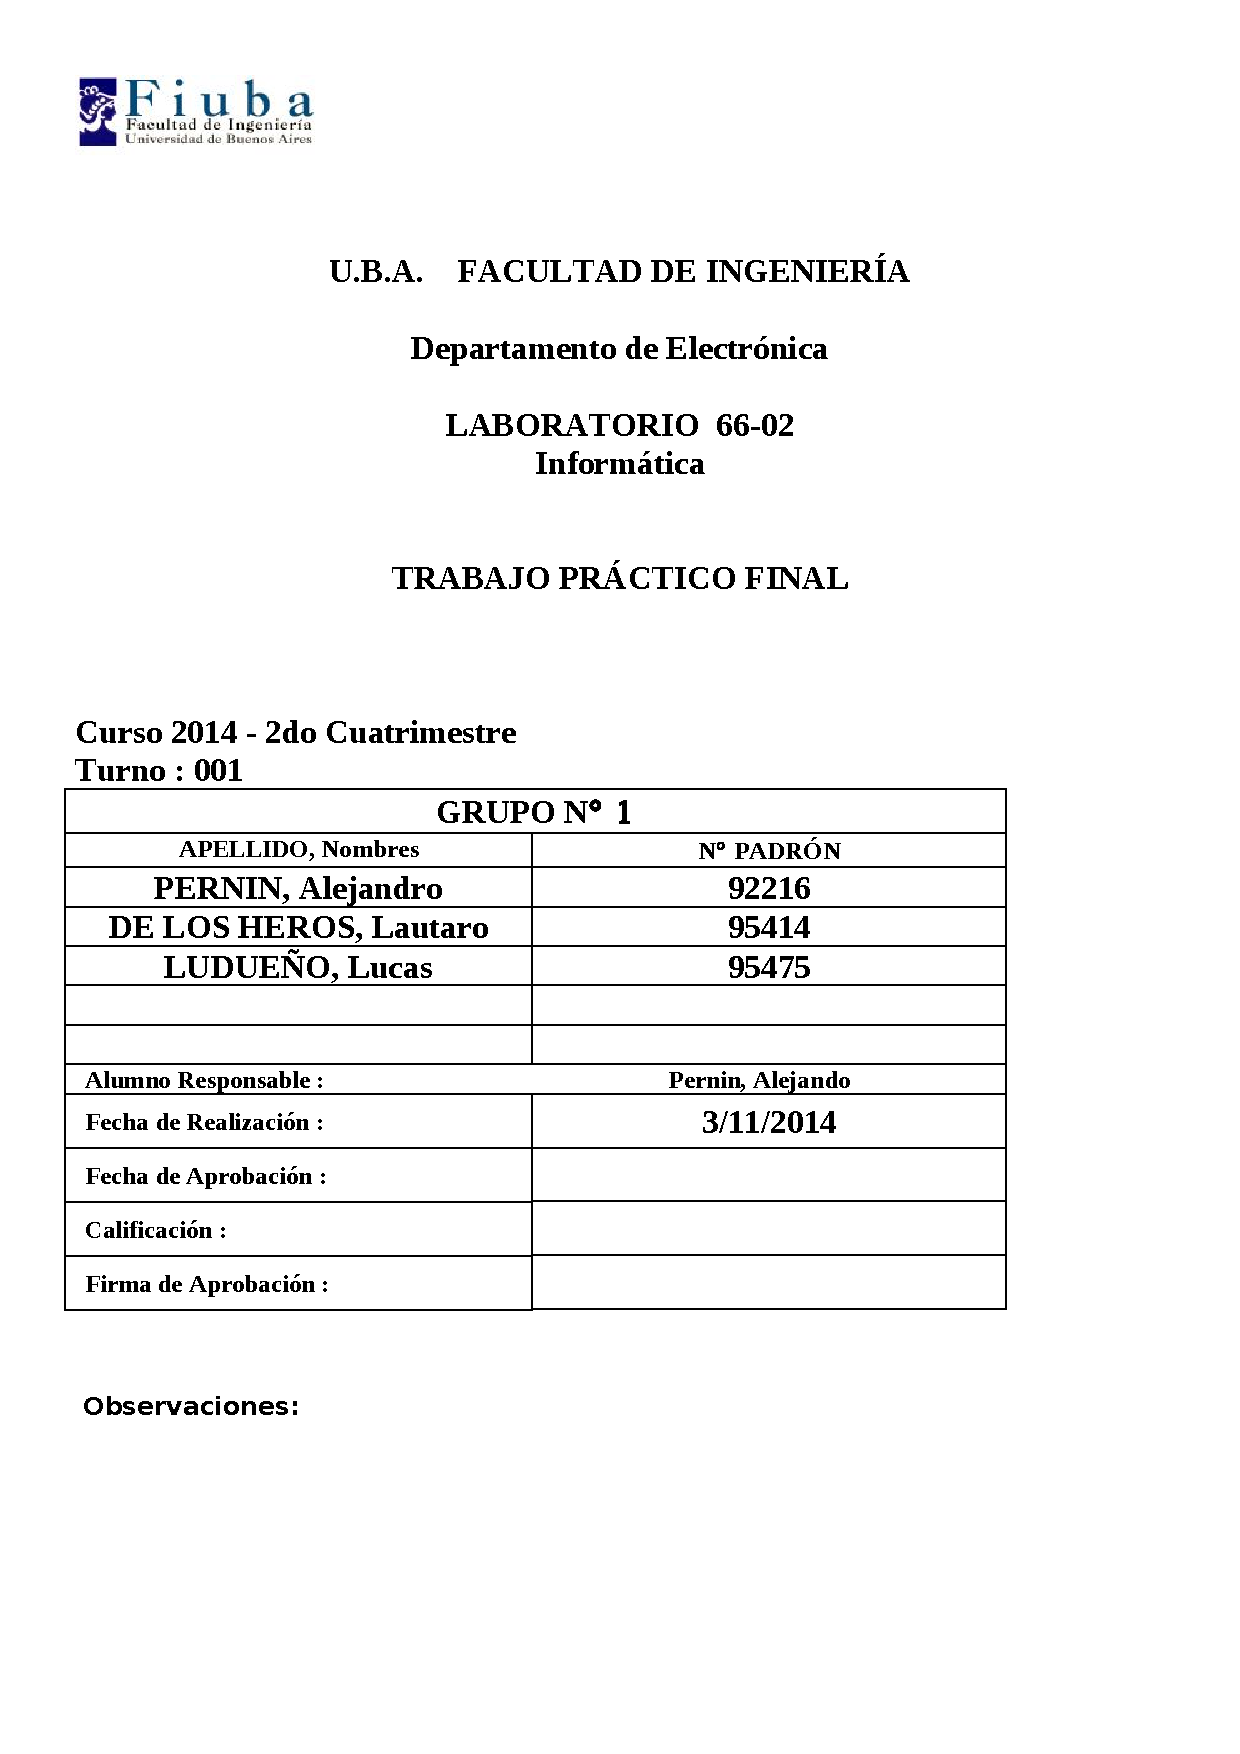
\includepdf{caratula.pdf}

\maketitle

\newpage
\tableofcontents

\newpage


\newpage 
\section{Introducción}
	El objetivo de este informe es exponer el trabajo práctico final, mostrando los desarrollos, mediciones efectuadas, funcionamiento y decisiones tomadas durante la confección del mismo. Éste fue realizado a lo largo del cuatrimestre en paralelo con las clases prácticas y los otros trabajos prácticos. Todos los archivo aquí utilizados, incluyendo este informe y su fuente estarán disponibles en \url{http://github.com/aleperno/labotpfinal}. \sout{Adicionalmente habrán disponibles algunos videos en YouTube con filmaciones de determinadas mediciones, por lo que es recomendable tener este informe en formato digital para fácil acceso a dichos links.}

	\subsection{Opciones Disponibles}
		Habiendo diversas alternativas de proyectos de TPs para elegir, en un principio no estuvo del todo claro cuál elegir ya que todos tenian sus complicaciones y objetivos. Algunas de las alternativas disponibles eran la confección de una fuente, un sensor, etc.

	\subsection{Opción Elegida}
		Como proyecto base decidimos desarrollar un voltímetro vúmetro disponible en los cursos de CEKIT \footnote{Pdf del proyecto oringal \url{https://github.com/aleperno/labotpfinal/raw/master/cekit.pdf}}. Elegimos este proyecto ya que si bien se trata de un proyecto relativamente sencillo, tiene aplicaciones reales tanto industriales como hogareñas.

		Además aprovechando que uno de los integrantes poseía un Arduino \footnote{\url{http://arduino.cc/}} y una Raspberry \footnote{\url{http://www.raspberrypi.org/}} decidimos como opcional escalar el proyecto utilizando dichos elementos. En el informe se desarrollará el proyecto base y el opcional se detallará en la sección \ref{sec:escalabilidad} de escalabilidad del proyecto.

		El vúmetro consiste en un arreglo de LEDs que se van encendiendo conforme aumenta la tensión mensurada, la relación entre la cantidad de LEDs encendidos y la tensión proviene de las características intrínsecas del circuito cuyo análisis es parte de este informe. En este proyecto no sólo se implementan las nociones aprendidas tanto en las clases teóricas  como en los TPs realizados, sino que además se emplearon nociones de diseño y elaboración de circuitos y software; por lo que es válido decir que este es un proyecto integrador.

	\newpage
	\section{Circuito Esquemático}
		El circuito implementado es el siguiente \footnote{.sch disponible en \url{https://github.com/aleperno/labotpfinal/raw/master/labo.sch}}:

		\begin{figure}[H]
			\centering
			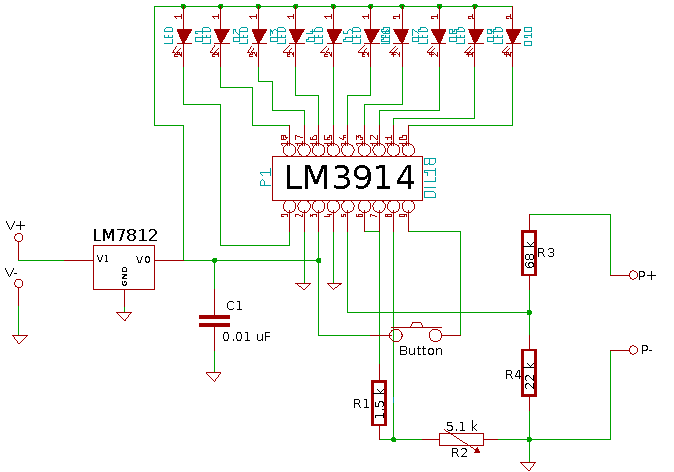
\includegraphics[scale=1.2]{images/sch.pdf}\caption{Esquemático del Circuito}
			\label{fig:circesq}
		\end{figure}

	\section{Diagrama de bloques}

		\begin{figure}[H]
			\centering
			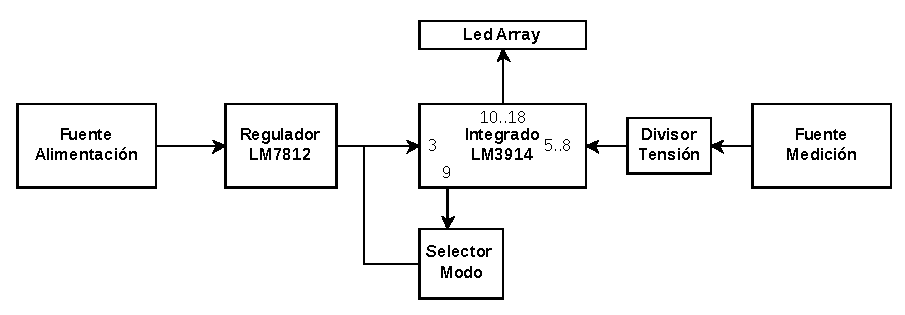
\includegraphics[scale=1.2]{images/bloque.pdf}\caption{Diagrama de Bloques}
			\label{fig:bloque}
		\end{figure}

	\begin{itemize}
		\item \textbf{Fuente de Alimentación:} La fuente que alimenta el circuito, ésta debe ser de al menos 14 V ya que el regulador de tensión es de 12V.
		\item \textbf{Regulador de Tensión:} El regulador cumple la función de mantener el equipo alimentado con 12 V, evitando daños si la entrada es mayor.
		\item \textbf{Selector Modo:} Nos permite seleccionar ambos modos de funcionamiento del circuito, tanto en "DOT" (se prende un sólo LED), como "BAR" (Se prende consecutivamente el array).
		\item \textbf{Fuente Medición:} Es la fuente de tensión a mensurar.
		\item \textbf{Divisor de Tensión:} Siendo que el integrado posee un límite de 5 V de entrada a medir, se coloca un divisor de tensión para ajustar la tensión a las especificaciones.
		\item \textbf{Array de LEDs:} Es el arreglo de LEDs luminosos en si, en este caso consiste de 10 LEDs.
		\item \textbf{Integrado LM3914: } Es el integrado encargado de la lógica del circuito.
	\end{itemize}

	\section{Desarrollo}
		Como primera instancia se debió analizar cuales serían los alcances del proyecto y ajustar las características del circuito al mismo. Lo principal a definir fue el rango de tensiones que mediriámos, decidimos utilizar el mismo rango utilizado como ejemplo en el proyecto orignal, comprendido entre los 0 y 25 V.

		Acorde al datasheet del integrado \footnote{Ver sección \ref{sec:referencias}.} el resistor $R_1$ es el encargado de regular la luminosidad de los LED. Asimismo se establece como corrientes de salida hacia los LED de un mínimo de 7 mA y un típico de 10 mA, para el proyecto establecimos un valor intermedio en $8.3$ mA. Siendo la tensión interna de referencia de $1.25$ V, por la ley de Ohm podemos calcular

		\begin{equation}
			R_1 = \frac{1.25 \: V * 10 \: LED}{8.3 \: mA} \cong 1.5 \: k \Omega
		\end{equation}

		Luego es preciso establecer un fondo de escala, la misma se calcula acorde la siguiente fórmula:

		\begin{equation}\label{eq:vref}
			V_{ref} = 1.25 \: V (1+\frac{R_2}{R_1})
		\end{equation}

		Siendo la máxima señal de entrada permitida de 5 V, para poder mensurar el rango antes mencionado (0 - 25 V) debemos emplear un divisor de tensión, para tal propósito se emplearon los resistores $R_3 = 68 \: k\Omega$ y $R_4 = 22 \: k\Omega$. Acorde a estos valores, aplicando una tensión de 25 V, sobre $R_4$ se obtendrá una caída de tensión equivalente a

		\begin{equation}
			\Delta V_{R_4} = \frac{25 \: V * 22 \: k\Omega}{90 \: k\Omega} \cong 6.1 \: V
		\end{equation}

		Si consideramos la tensión máxima de referencia, según la ecuacion \ref{eq:vref}:

		\begin{equation}
			\displaystyle R_2 = \left.  \left ( \frac{V_{ref}}{1.25 \: V}-1 \right ) * R_1 \right |_{V_{ref} = 5 \: V} = 4.5 \: k\Omega
		\end{equation}

		Siendo este resistor de un valor no comercial y con el fin de a posteriori poder realizar ajustes, empleamos un resistor variable de $10 \: k\Omega$. Teniendo todos los elementos principales ya descriptos, se prosiguió al diseño y confección del circuito.

		%Sin embargo al tener también interactuando un divisor de tensión (y resistores no exactos), empleamos un resistor variable de $10 \: k\Omega$ y aplicando una tensión de 25 V variamos la resistencia, procurando que a los 25 V se encienca el décimo LED. Una vez hecho esto, se midió la resistencia del resistor dando como resultado:

		%\begin{equation}
		%	R_2 = (3.87 \pm 0.05) \: k\Omega
		%\end{equation}

		\subsection{Construcción}

			Como primer instancia luego de adquirir todos los elementos, se armó el circuito en un \textit{protoboard} a fin de corroborar el funcionamiento de todos los componentes individual y conjuntamente.

			\begin{figure}[H]
			\centering
				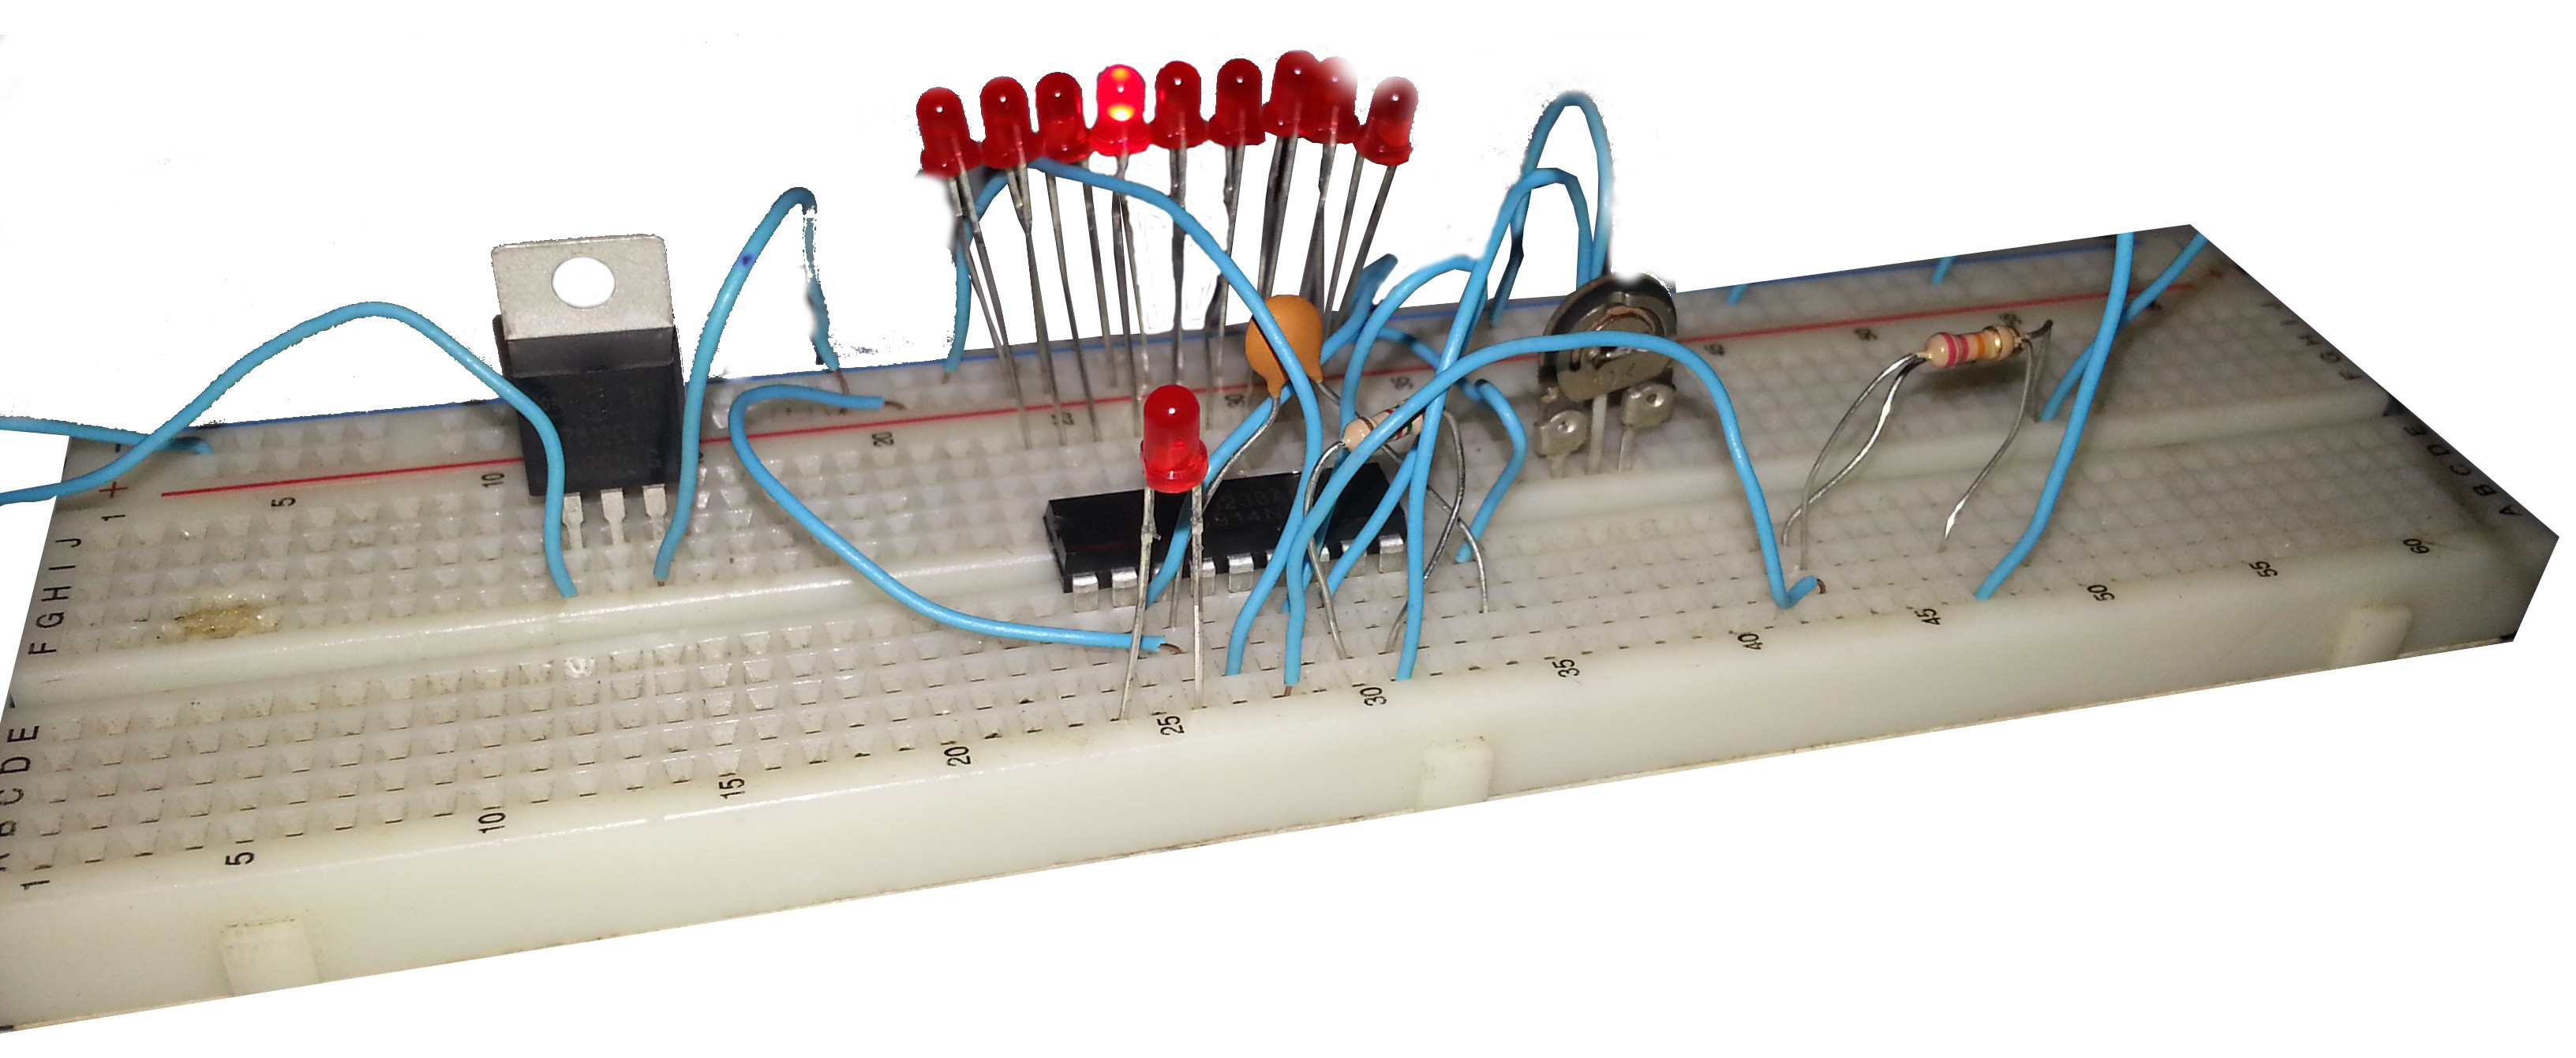
\includegraphics[scale=0.1]{images/proto_dot.jpg}\caption{Prototipo modo DOT}
			\end{figure}

			\begin{figure}[H]
			\centering
				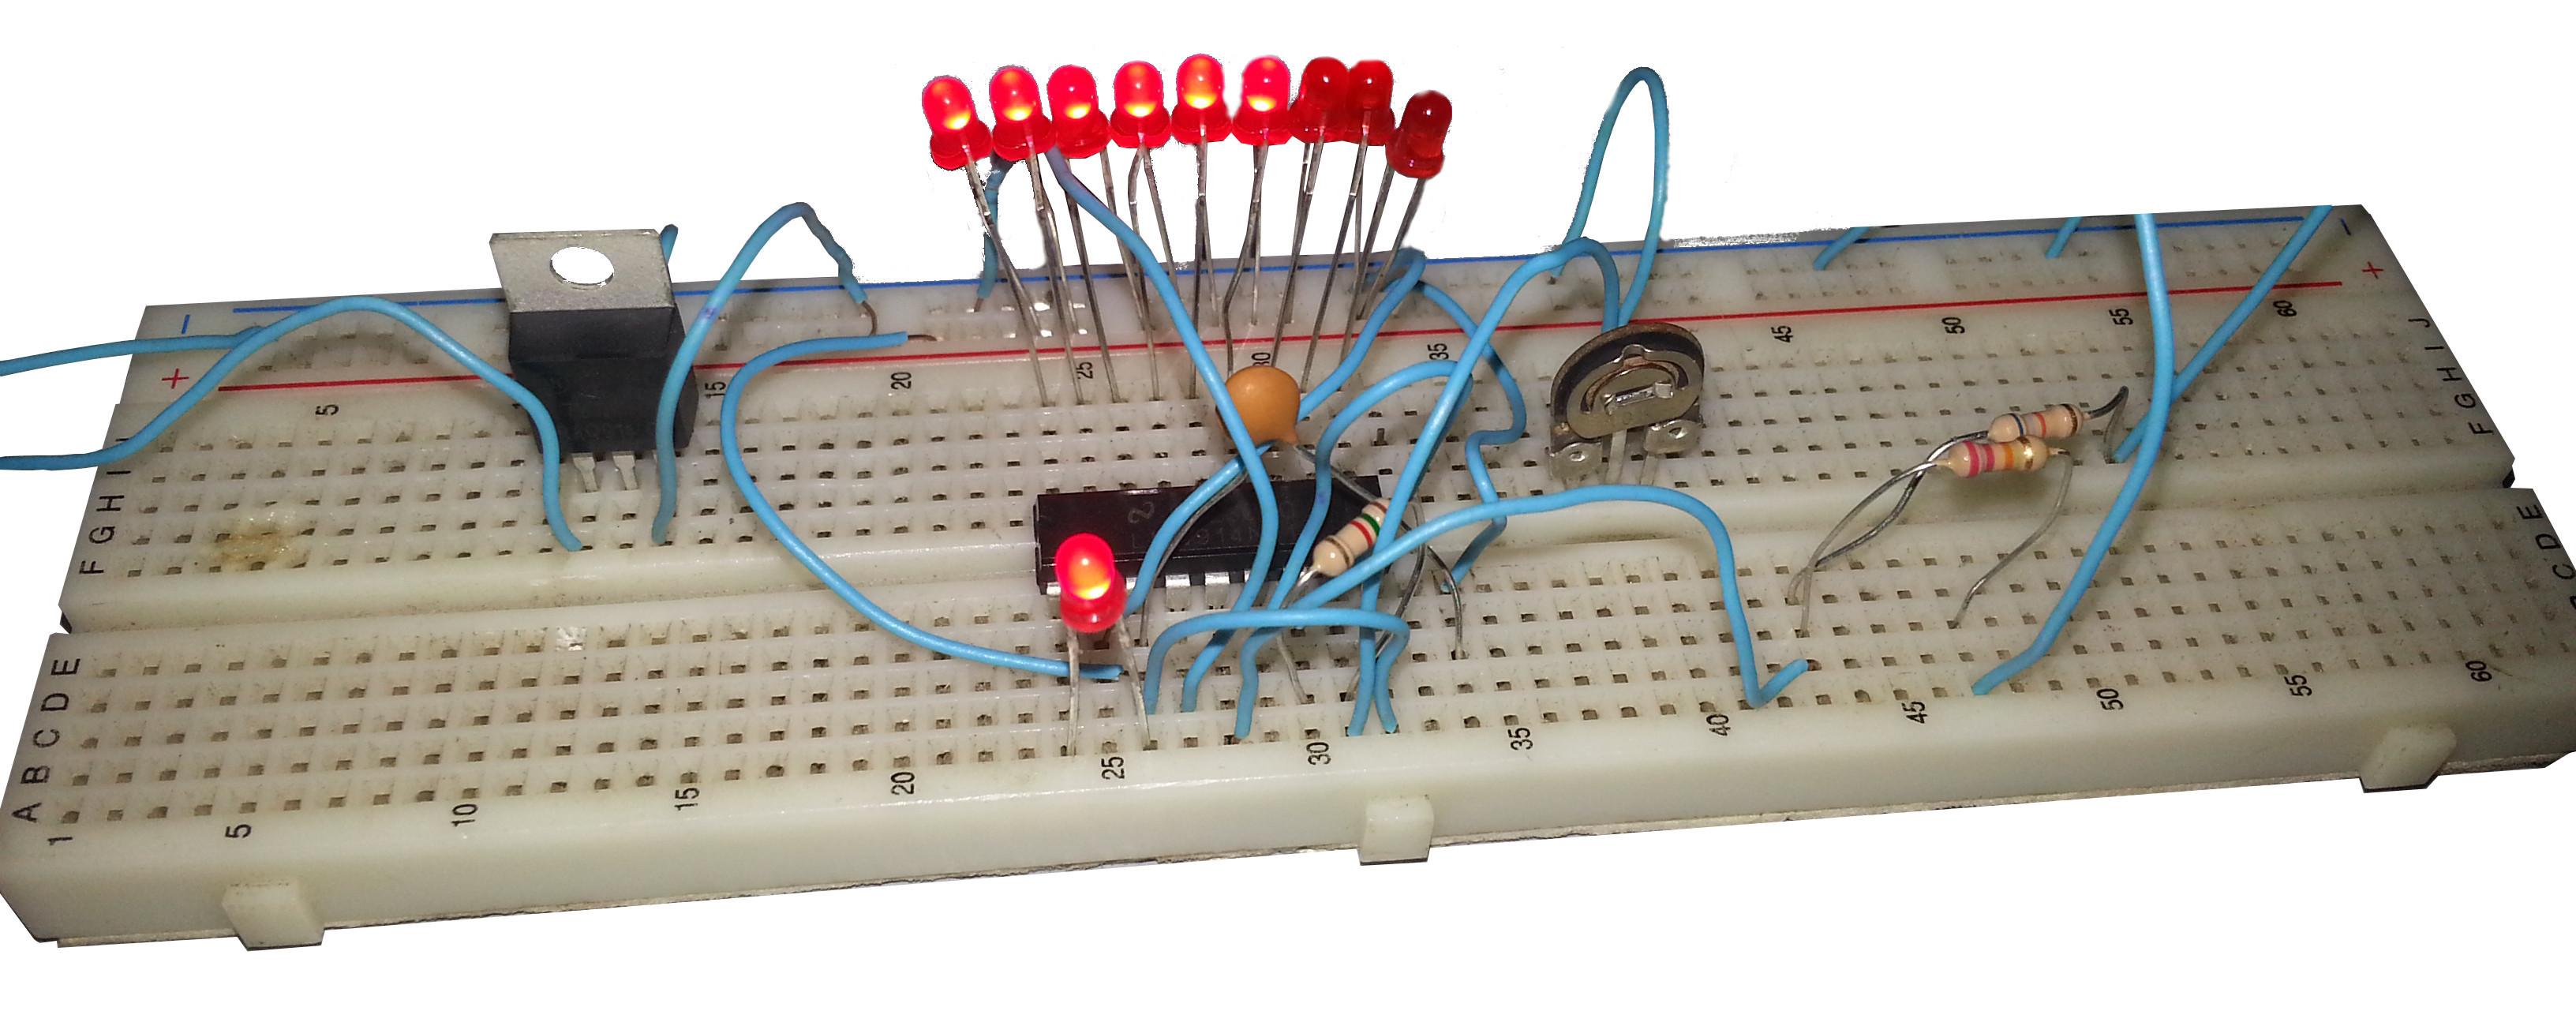
\includegraphics[scale=0.1]{images/proto_bar.jpg}\caption{Prototipo modo BAR}
			\end{figure}

			Luego aprovechando la disponibilidad de un archivo esquemático, utilizando herramientas informáticas se diseñó un circuito virtual que luego sería pasado a una plaqueta de cobre.

			\begin{figure}[H]
			\centering
				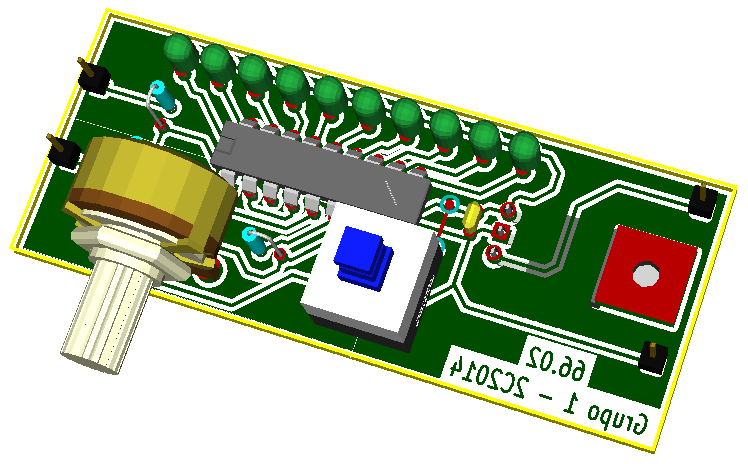
\includegraphics[scale=0.4]{images/virt_sup.png}\caption{Vista Superior Circuito Virtual}
			\end{figure}

			\begin{figure}[H]
			\centering
				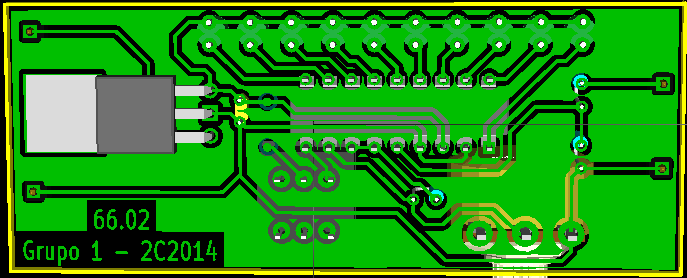
\includegraphics[scale=0.4]{images/virt_inf.png}\caption{Vista Inferior Circuito Virtual}
			\end{figure}

			Una vez conformes con el diseño, se imprimió el mismo en papel de transferencia térmico, para ser pasado a una plancha de cobre virgen y empleando ácido grabar el dibujo en la placa.

			\begin{figure}[H]
			\centering
				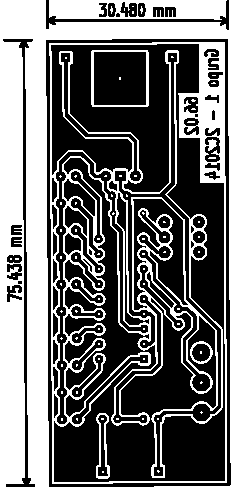
\includegraphics[scale=1,angle=-90]{images/design.pdf}\caption{Diseño Circuito}
			\end{figure}

			\begin{figure}[H]
			\centering
				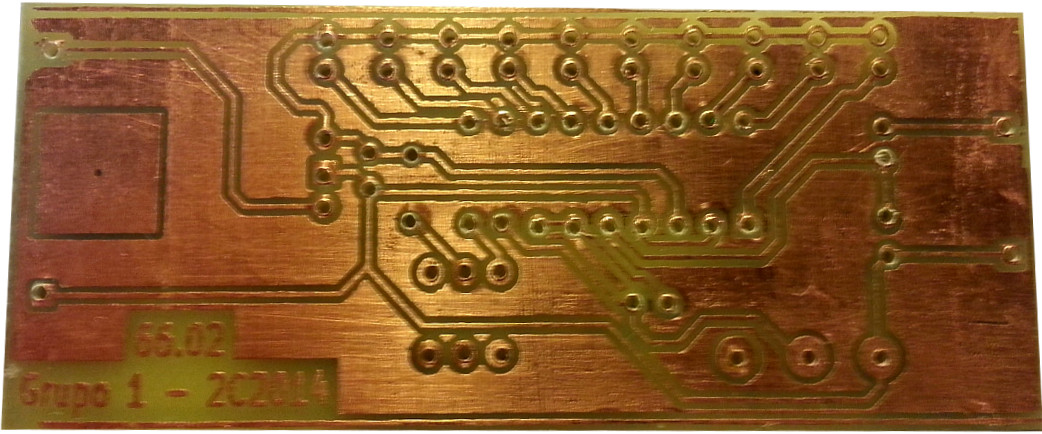
\includegraphics[scale=0.25]{images/placa_grabada.jpg}\caption{Diseño Grabado}
			\end{figure}

			\begin{figure}[H]
			\centering
				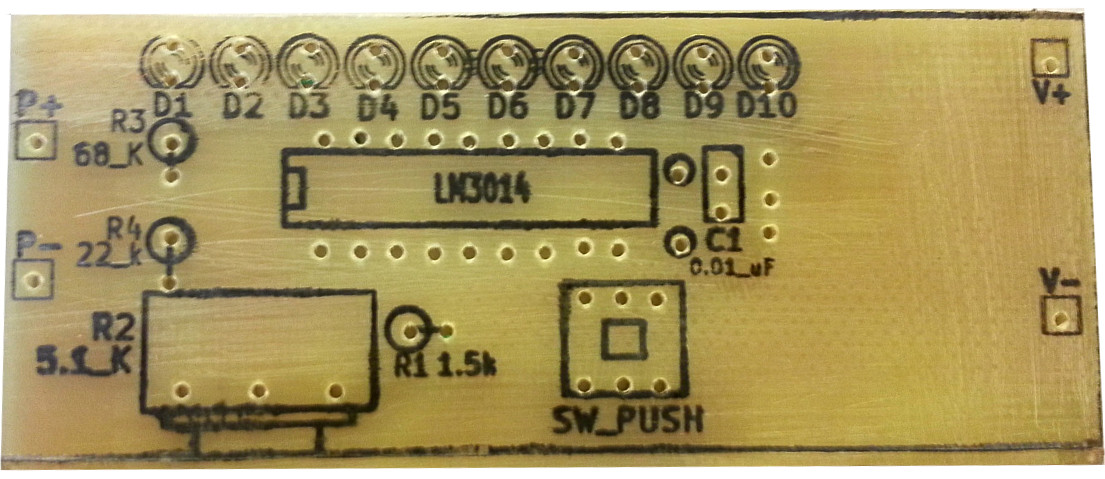
\includegraphics[scale=0.25]{images/ayuda_comps.jpg}\caption{Indicador de Componentes}
			\end{figure}

			Luego de soldar los componentes y realizar algunas reparaciones en las pistas de cobre, el circuito definitivo:

			\begin{figure}[H]
			\centering
				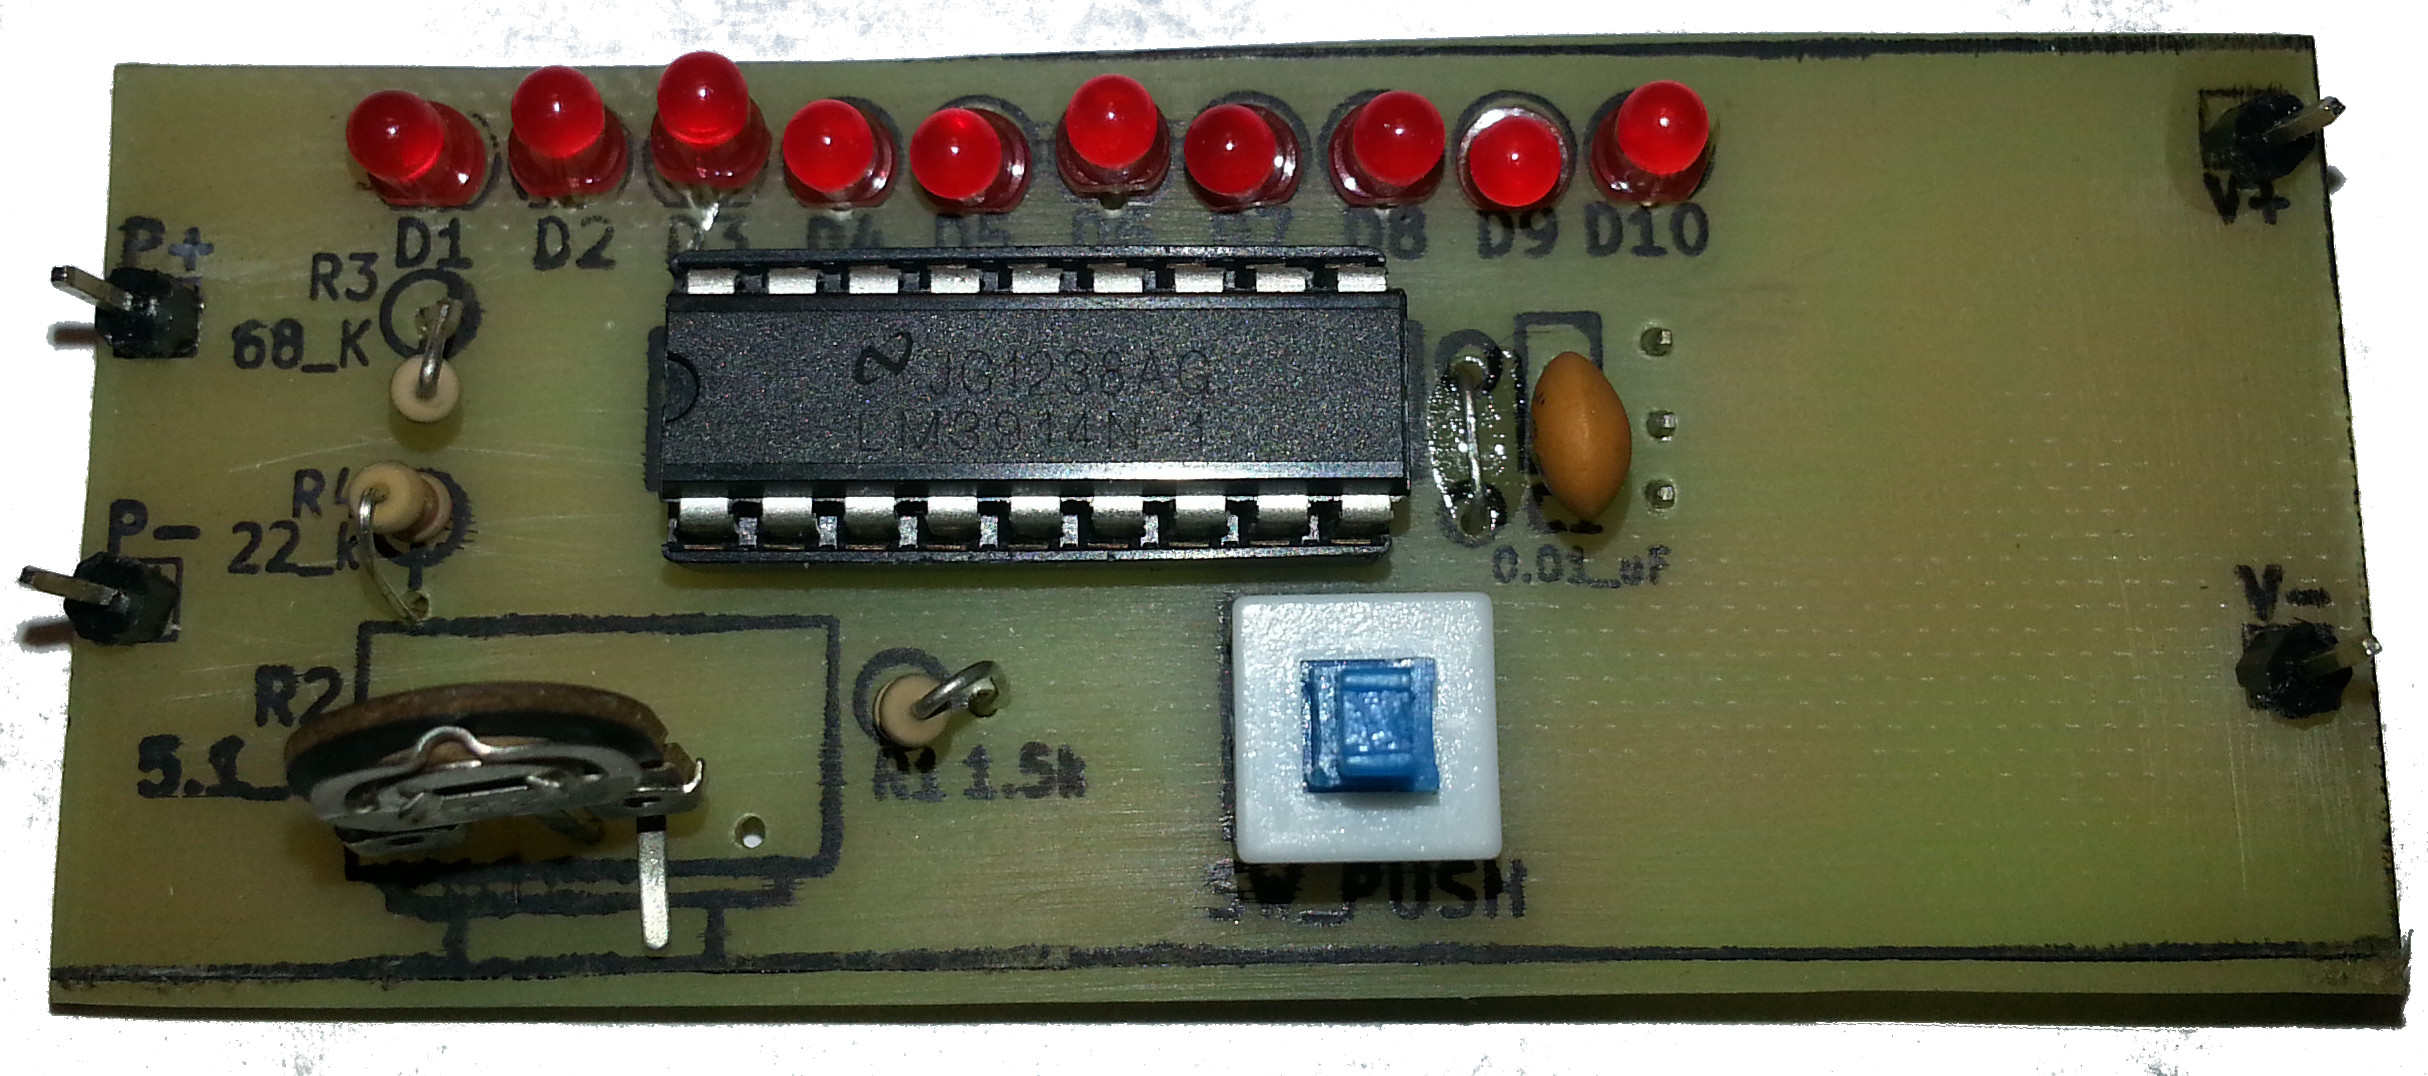
\includegraphics[scale=0.1]{images/placa_completa.jpg}\caption{Circuito Completo}
			\end{figure}

		\subsection{Materiales y Costo}

		\begin{center}
			
			{\footnotesize \begin{tabular}{ |c|l|r|r| }

			\hline
				\multicolumn{4}{|c|}{\textbf{Materiales}}\\ \hline
				Cantidad & Descripción & Precio Unitario [\$] & Subtotal [\$] \\ \hline
				1 & Resistor $1.5 \: k\Omega$ & $0.25$ & $0.25$\\ \hline
				1 & Resistor variable $10 \: k\Omega$ & $8$& $8$ \\ \hline
				1 & Resistor $68 \: k\Omega$ & $0.25$&$0.25$ \\ \hline
				1 & Resistor $22 \: k\Omega$ & $0.25$& $0.25$\\ \hline
				10 & LED Rojo 3 mm & $1.5$ & $15$\\ \hline
				1 & Capacitor Cerámico $0.01 \: \mu F$ & $1$& $1$\\ \hline
				1 & Pulsador 6 pines & $5$ & $5$ \\ \hline
				1 & Integrado LM3914 & $28$ & $28$\\ \hline
				1 & Regulador LM7812 & $5.5$& $5.5$ \\ \hline
				1 & Base Integrado 18 pines & $2$& $2$ \\ \hline
				1 & Placa Cobre 10x10 cm & $9$& $9$ \\ \hline
				1 & Hoja Transferencia Térmica & 10 & 10\\ \hline
				\multicolumn{4}{|r|}{Total:  $84.25$}\\ \hline


			\end{tabular}}\captionof{table}{Lista de Precios}\label{tab:costo}
			\end{center}

		\subsection{Mediciones}

			Siendo que para la realización de mediciones el circuito impreso no resulta muy apropiado por la dificultad (o imposibilidad) de conectar los terminales de los voltímetros se optó por emplear toda otra serie de compuestos en un \textit{protoboard} para así facilitar ciertas mediciones.

			\begin{figure}[H]
			\centering
				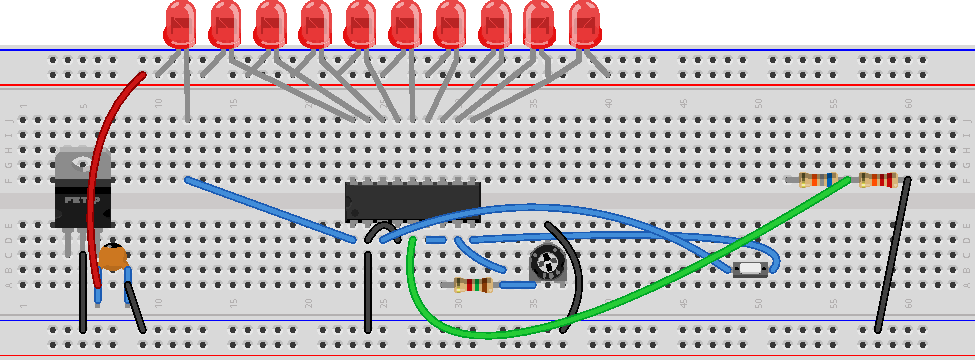
\includegraphics[scale=1]{images/proto.pdf}\caption{Protoboard}\label{fig:proto}
			\end{figure}

			Para todas las mediciones a realizar se empleará el multímetro digital MS8221A utilizado en los trabajos anteriores, en caso de emplearse otro se aclarará explícitamente. Asímismo las fuentes reguladas a utilizar serán las HY3005D empleadas con anterioridad, para el funcionamiento de este proyecto se emplearán dos, una como alimentación del circuito y otra como fuente a mensurar.

			\subsubsection{Regulador}

			Uno de los componentes claves del circuito es el regulador de tensión LM7812, el cual se emplea con el propósito de obtener una salida constante de 12 V. Como primera medición se mide la salida del regulador respecto de la entrada de tensión. Se espera que a bajos voltajes la tensión de salida sea similar a la tensión de entrada pero menor. Además se espera que la tensión para la cual la salida se estabiliza, este uno o dos voltios por encima de los 12 V.

			Empleando un simple banco de medición con una fuente y un voltímetro se obtuvieron los siguientes datos.

			\begin{figure}[H]
			\centering
				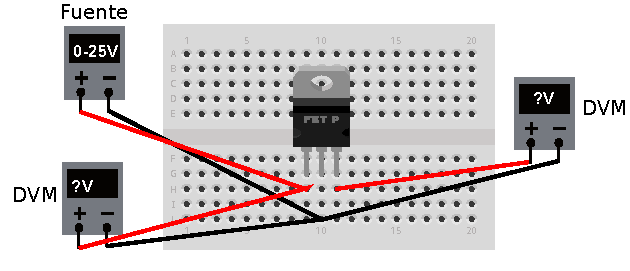
\includegraphics[scale=1]{images/reg.pdf}\caption{Banco de Medición Regulador de Tensión}\label{fig:banco0}
			\end{figure}

			\begin{center}
			{\footnotesize \begin{tabular}{ |l|l|l|l| }

			\hline
				\multicolumn{4}{|c|}{\textbf{Regulador Tensión}}\\ \hline
				$V_{in}$ & $\Delta V_{in}$ & $V_{out}$ & $\Delta V_{out}$ \\ \hline
				$1.62$ & $0.02$ & $0.97$ & $0.02$\\ \hline
				$3.24$ & $0.03$ & $2.55$ & $0.02$\\ \hline
				$4.96$ & $0.04$ & $4.2$ & $0.04$\\ \hline
				$7.56$ & $0.05$ & $6.75$ & $0.05$\\ \hline
				$10.34$ & $0.07$ &  $9.5$ & $0.05$\\ \hline
				$12.44$ & $0.08$ & $11.58$ & $0.07$\\ \hline
				$12.76$ & $0.08$ & $11.91$ & $0.07$\\ \hline
				$13$ & $0.08$ & $12.14$ & $0.08$\\ \hline
				$13.13$ & $0.08$ & $12.2$ & $0.08$\\ \hline
				$13.37$ & $0.08$ & $12.21$ & $0.08$\\ \hline
				$14.36$ & $0.09$ & $12.21$ & $0.08$\\ \hline
				$15.75$ & $0.09$ & $12.21$ & $0.08$ \\ \hline
				$17.38$ & $0.10$ & $12.22$ & $0.08$\\ \hline
				$20.1$ & $0.3$ &  $12.21$ & $0.08$ \\ \hline
				$22.4$ & $0.3$ &  $12.21$ & $0.08$ \\ \hline
				$24.5$ & $0.3$ &  $12.21$ & $0.08$ \\ \hline
				$28.1$ & $0.3$ &  $12.22$ & $0.08$ \\ \hline
				$31.4$ & $0.3$ &  $12.25$ & $0.08$ \\ \hline			
 				
				
			\end{tabular}}\captionof{table}{Medición LM7812}\label{tab:regtension}
			\end{center}

			\begin{figure}[H]
			\centering
				\includegraphics[scale=0.035]{images/med_reg.pdf}\caption{Tensión Salida Regulador}\label{fig:grafreg}
			\end{figure}

			Como era de esperarse, la tensión de salida es lineal e inferior a la tensión de entrada a tensiones bajas. También confirmamos que el punto en el cuál la tensión de salida se estabiliza (13.13 V) se encuentra por encima de la tensión de regulación. La figura \ref{fig:grafreg} no posee barras de errores ya que como se puede apreciar en el cuadro \ref{tab:regtension} los errores son despreciables respectos de los valores que operamos.

			\subsubsection{Escala}
				Acorde a las hipótesis realizadas, el vúmero posee un fondo de escala de 25 V distribuidos en 10 LEDs, por lo que cada LED representará un aumento en la tensión de 2,5 V. 

				\begin{center}
			{\footnotesize \begin{tabular}{ |c|l| }

			\hline
				\multicolumn{2}{|c|}{\textbf{Escala LEDs}}\\ \hline
				$\#$Led Encendido(s) & Tensión [V] \\ \hline
				$0$ & $< 2.5$ \\ \hline
				$1$ & $2.5$ \\ \hline
				$2$ & $5$ \\ \hline
				$3$ & $7.5$ \\ \hline
				$4$ & $10$ \\ \hline
				$5$ & $12.5$ \\ \hline
				$6$ & $15$ \\ \hline
				$7$ & $17.5$ \\ \hline
				$8$ & $20$ \\ \hline
				$9$ & $22.5$ \\ \hline
				$10$ & $25$ \\ \hline			
 				
				
			\end{tabular}}\captionof{table}{Escala leds}\label{tab:escala}
			\end{center}

			Para corrobororar esta escala y/o realizar los ajustes necesarios se emplearon dos fuentes reguladas, una como fuente de alimentación del circuito y otra como fuente a mensurar. Asimismo en paralelo con la fuente a mensurar se coloca un multímetro digital a fin de tener una lectura mas exacta de la tensión respecto de la mostrada por la pantalla LED de la fuente.

			\begin{figure}[H]
			\centering
				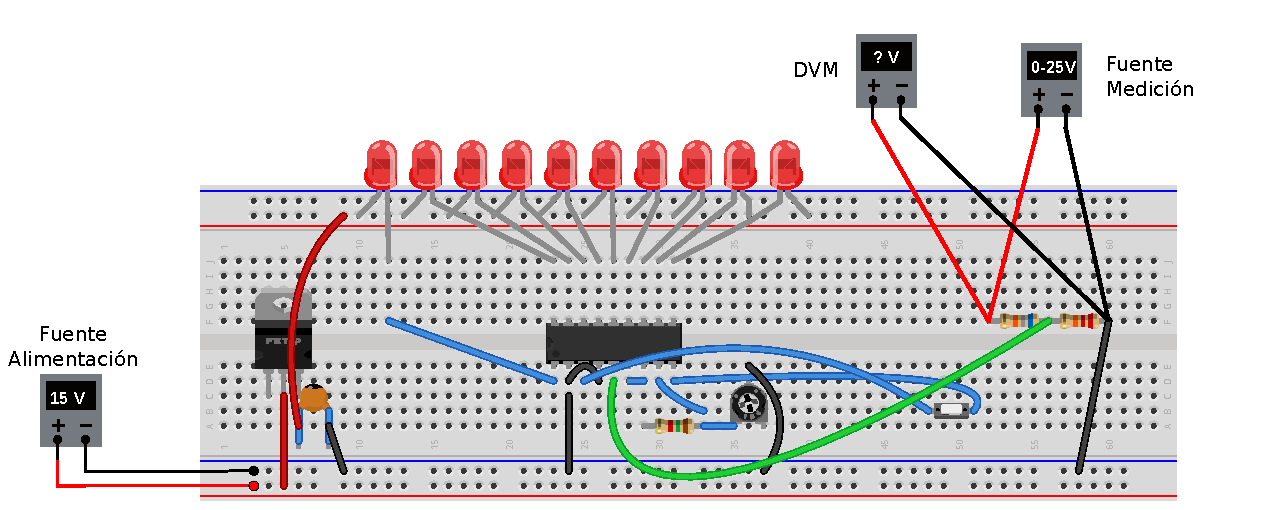
\includegraphics[scale=0.8]{images/banco1.pdf}\caption{Banco de Medición Escala}\label{fig:banco1}
			\end{figure}

			\subsubsection{Consumo}
				Una de las principales características de este circuito, es la capacidad de cambiar entre modo BAR y modo DOT, obteniendo así una misma lectura expresada en un sólo led o en un continuo de leds. A priori se puede deducir que entre ambos modos habrá una diferencia de consumo proveniente de tener un sólo led o un número de leds. Asímismo se espera que en modo punto el consumo sea lineal, para ello se fue variando la tensión de la fuente a mensurar y se midió la corriente. Con dichos valores se calculó la potencia.

				\begin{center}
			
			{\footnotesize \begin{tabular}{ |l|l|l|l|l|l| }

			\hline
				\multicolumn{6}{|c|}{\textbf{Mediciones DOT}}\\ \hline
				Tensión [V] & $\Delta V$ [V] & Corriente [mA] & $\Delta I$ [mA] & Consumo [mW] & $\Delta$ Consumo [mW]\\ \hline
				$0.40$ & $0.02$ & $10.2$ & $0.3$ & $4.1$ & $0.3$ \\ \hline
				$1.29$ & $0.02$ & $10.2$ & $0.3$ & $13.2$ & $0.5$ \\ \hline
				$2.50$ & $0.03$ & $24.3$ & $0.4$ & $60.8$ & $1.6$ \\ \hline
				$3.82$ & $0.03$ & $24.4$ & $0.4$ & $93.2$ & $2.3$ \\ \hline
				$5.08$ & $0.04$ & $24.3$ & $0.4$ & $123.4$ & $2.9$ \\ \hline
				$6.78$ & $0.05$ & $24.3$ & $0.4$ & $164.8$ & $3.8$ \\ \hline
				$7.50$ & $0.05$ & $23.7$ & $0.4$ & $177.8$ & $4.1$ \\ \hline
				$8.85$ & $0.06$ & $23.8$ & $0.4$ & $210.6$ & $4.8$ \\ \hline
				$10.61$ & $0.07$ & $24.5$ & $0.4$ & $259.9$ & $5.8$ \\ \hline
				$11.83$ & $0.07$ & $24.4$ & $0.4$ & $288.7$ & $6.4$ \\ \hline
				$12.64$ & $0.08$ & $24.4$ & $0.4$ & $308.4$ & $6.8$ \\ \hline
				$13.81$ & $0.08$ & $24.4$ & $0.4$ & $337.0$ & $7.4$ \\ \hline
				$15.08$ & $0.09$ & $24.1$ & $0.4$ & $363.4$ & $8.0$ \\ \hline
				$16.75$ & $0.1$ & $24.1$ & $0.4$ & $403.7$ & $8.8$ \\ \hline
				$17.63$ & $0.1$ & $24.0$ & $0.4$ & $423.1$ & $9.2$ \\ \hline
				$18.75$ & $0.1$ & $24.0$ & $0.4$ & $450.0$ & $9.8$ \\ \hline
				$20.0$ & $0.2$ & $23.7$ & $0.4$ & $474.0$ & $10.3$ \\ \hline
				$21.3$ & $0.2$ & $23.7$ & $0.4$ & $504.8$ & $11.0$ \\ \hline
				$22.5$ & $0.2$ & $23.9$ & $0.4$ & $537.8$ & $11.7$ \\ \hline
				$23.7$ & $0.2$ & $23.9$ & $0.4$ & $566.4$ & $12.3$ \\ \hline
				$25.0$ & $0.2$ & $24.0$ & $0.4$ & $600.0$ & $13.0$ \\ \hline
				$26.4$ & $0.2$ & $24.0$ & $0.4$ & $633.6$ & $13.7$ \\ \hline
 				
				
			\end{tabular}}\captionof{table}{Medición Consumo modo DOT}\label{tab:consumodot}
			\end{center}

			\begin{center}
			{\footnotesize \begin{tabular}{ |l|l|l|l|l|l| }

			\hline
				\multicolumn{6}{|c|}{\textbf{Mediciones BAR}}\\ \hline
				Tensión [V] & $\Delta V$ [V] & Corriente [mA] & $\Delta I$ [mA] & Consumo [mW] & $\Delta$ Consumo [mW]\\ \hline
				$0.40$  & $0.02$ & $ 10.3 $ &  $ 0.3 $ & $ 4.1 $   & $ 0.3 $ \\ \hline
				$1.29$  & $0.02$ & $ 10.3$ &   $ 0.3 $ & $ 13.3 $  & $ 0.5 $ \\ \hline
				$2.50$  & $0.03$ & $ 24.5 $ &  $ 0.4 $ & $ 61.3 $  & $ 1.6 $ \\ \hline
				$3.82$  & $0.03$ & $ 24.5 $ &  $ 0.4 $ & $ 93.6 $  & $ 2.3 $ \\ \hline
				$5.08$  & $0.04$ & $ 38.5 $ &  $ 0.6 $ & $ 195.6 $ & $ 4.3 $ \\ \hline
				$6.78$  & $0.05$ & $ 38.5 $ &  $ 0.6 $ & $ 261.0 $ & $ 5.6 $ \\ \hline
				$7.50$  & $0.05$ & $ 51.8 $ &  $ 0.8 $ & $ 388.5 $ & $ 7.9 $ \\ \hline
				$8.85$  & $0.06$ & $ 51.8 $ &  $ 0.8 $ & $ 458.4 $ & $ 9.2 $ \\ \hline
				$10.61$ & $0.07$ & $ 65.7 $ &  $ 0.9 $ & $ 697.1 $ & $ 13.6 $ \\ \hline
				$11.83$ & $0.07$ & $ 65.7 $ &  $ 0.9 $ & $ 777.2 $ & $ 15.1 $ \\ \hline
				$12.64$ & $0.08$ & $ 79.6 $ &  $ 1.1 $ & $ 1006.1 $ & $ 19.2 $ \\ \hline
				$13.81$ & $0.08$ & $ 79.6 $ &  $ 1.1 $ & $ 1099.3 $ & $ 20.9 $ \\ \hline
				$15.08$ & $0.09$ & $ 93.4$ &   $ 1.3 $ & $  1408.5$ & $ 26.4 $ \\ \hline
				$16.75$ & $0.1$  & $ 93.4 $ &  $ 1.3 $ & $ 1564.5 $ & $ 29.3 $ \\ \hline
				$17.63$ & $0.1$  & $ 107.3 $ & $ 1.4 $ & $ 1891.7 $ & $ 35.0 $ \\ \hline
				$18.75$ & $0.1$  & $ 107.3 $ & $ 1.4 $ & $ 2011.9 $ & $ 37.2 $ \\ \hline
				$20.0$  & $0.2$  & $ 120.4 $ & $ 1.6 $ & $ 2408.0 $ & $ 44.2 $ \\ \hline
				$21.3$  & $0.2$  & $ 120.5 $ & $ 1.6 $ & $ 2566.7 $ & $ 47.0 $ \\ \hline
				$22.5$  & $0.2$  & $ 133.0 $ & $ 1.7 $ & $ 2992.5 $ & $ 54.5 $ \\ \hline
				$23.7$  & $0.2$  & $ 133.1 $ & $ 1.7 $ & $ 3154.5 $ & $ 57.4 $ \\ \hline
				$25.0$  & $0.2$  & $ 145.0 $ & $ 1.9 $ & $ 3625.0 $ & $ 65.6 $ \\ \hline
				$26.4$  & $0.2$  & $ 145.2 $ & $ 1.9 $ & $ 3833.3 $ & $ 69.3 $ \\ \hline
 				
				
			\end{tabular}}\captionof{table}{Medición Consumo modo BAR}\label{tab:consumobar}
			\end{center}

			Con toda esta información disponible, es posile comparar mediante gráficos y confirmar algunas deducciones.

			\begin{figure}[H]
			\centering
				\includegraphics[scale=0.03]{images/corriente.pdf}\caption{Corriente vs Tensión}\label{fig:corriente}
			\end{figure}

			Como era de esperarse, la corriente en modo punto es constante observándose sólo un salto siendo que antes de los $2.5 \:V$ no se encuentra ningun led encendido. Asimismo se observa que en modo bar la corriente es lineal, habiendo unos descansos correspondientes a tensiones dentro del rango de un mismo led. 

			Una interrogante que se puede desprender de este gráfico es si dichos saltos son constantes.

			\begin{figure}[H]
			\centering
				\includegraphics[scale=0.03]{images/salto.pdf}\caption{Saltos Corriente}
			\end{figure}

			Estos saltos corresponden al valor de una corriente respecto de la corriente antes mensurada. Otra vez es observable como en modo punto sólo hay un salto y luego los saltos se encuentran muy próximos a 0. Para el modo bar, se observa una oscilacion correspondiente a que los puntos dentro del mismo rango de tension de un led (eg: 2,6 V y 3.0 V encienden el mismo led) no hay salto de corriente significativo, pero al encender un nuevo led si. Asimismo es visible como los valores pico de estos saltos se mantienen dentro de un rango discreto.

			\begin{figure}[H]
			\centering
				\includegraphics[scale=0.03]{images/pot.pdf}\caption{Potencia}\label{fig:potencia}
			\end{figure}

			Es observable como la potencia disipada por el circuito en modo BAR no sólo es mayor al de modo DOT punto a punto, sino también como la curva de crecimiento de la misma tiene a una forma exponencial. Esto tiene sentido ya que considerando la potencia como

			\begin{equation}
				P = V * I
			\end{equation}
			donde $P$, $V$ e $I$ son la potencia, tensión y corriente respectivamente; de ser la corriente constante la potencia describirá una curva lineal tal cual indica la figura \ref{fig:potencia} para el modo DOT. En el caso del modo BAR, la corriente incrementa linealmente respecto de la tensión (ver figura \ref{fig:corriente}) pudiéndola expresar como $I = \alpha V$, siendo $\alpha$ una constante de proporción. Aplicando esto a la ecuación arriba descripta

			\begin{equation}
				P = V * I = V * \alpha V = \alpha V^2 
			\end{equation}
			lo que valida que la curva describa una trayectoria exponencial.

	\newpage
	\section{Escalabilidad}	\label{sec:escalabilidad}

		Pensando en las aplicaciones prácticas de un voltímetro, nos encontramos con la necesidad de poder obtener una lectura exacta y/o a distancia. Un vúmetro si bien es de lectura sencilla, no nos da un valor númerico ni tampoco nos permite leer la lectura a distancia. Si pensamos esto a nivel industrial es una gran desventaja, quizá por cuestiones de la complejidad de un determinado proceso es preciso obtener una lectura exacta; asimismo las extensiones de las plantas industriales obligan a realizar mediciones mediante sensores que reporten a una base central, para consultarlas en un centro de control.

		Abstrayendonos del caso insdustrial planteado y aprovechando que un compañero poseía un Arduino y Raspberry, decidimos implementar un voltímetro que muestre en una pantalla LED la tensión mensurada y asímismo permita una lectura a distancia. Para ello utilizamos un Arduino Mega 2560 R3 \footnote{\url{http://arduino.cc/en/Main/arduinoBoardMega} } con un \textit{shield} LCD DFRobot\footnote{\url{http://www.dfrobot.com/wiki/index.php?title=Arduino_LCD_KeyPad_Shield_(SKU:_DFR0009)} } y una Raspberry Pi B+ \footnote{\url{http://www.raspberrypi.org/products/model-b-plus/} }.

		En nuestro caso el Arduino actuará como sensor, que no sólo tomará las mediciones sino que las mostrará en una pantalla LCD sino que también las comunicará a la Raspberry por puerto serie. La Raspberry representará un sistema central de obtención de mediciones, en la misma se instaló un servidor web Apache y una simple página en PHP que muestra vía web las tensiones mensuradas en tiempo real. Además esta configuración nos permitiría registrar un historial de las mediciones realizadas para posterior análisis.

		Utilizando el mismo rango de tensiones utilizado con el vúmetro y siendo la máxima tensión permitida por el Arduino de 5 V es necesario utilizar un resistor de tensión, para lo cuál se utilizaron resistores de $100 \: \Omega$ y $1 \: k\Omega$. 

		\begin{figure}[H]
			\centering
				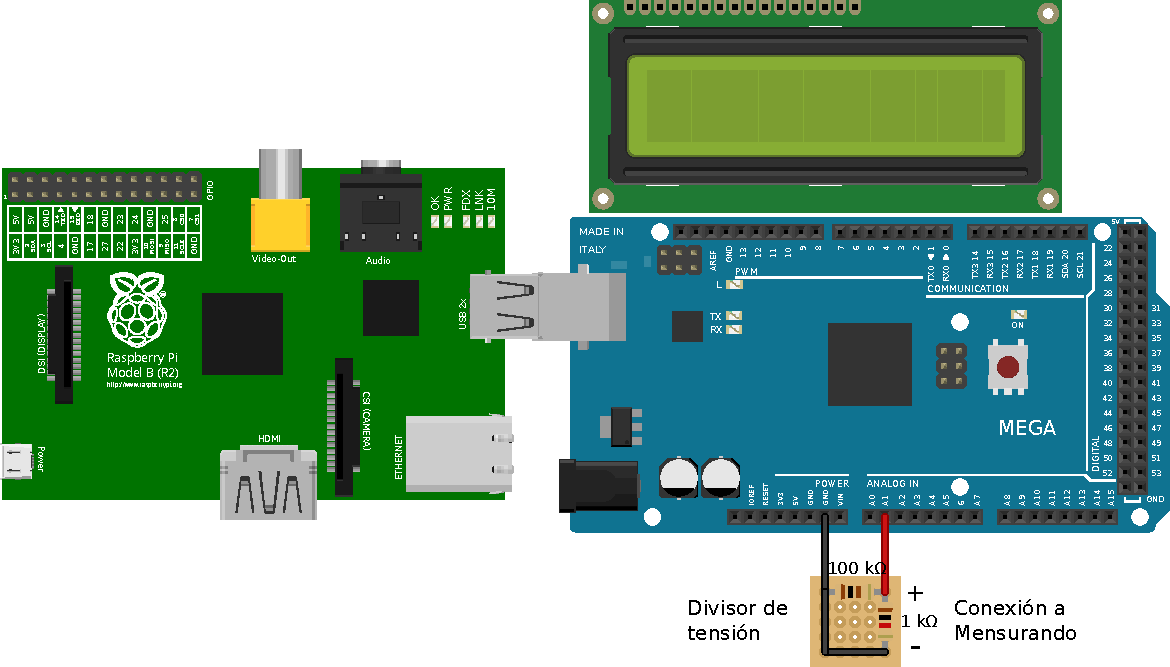
\includegraphics[scale=0.8]{images/arduino1.pdf}\caption{Banco Medición Arduino - Raspberry}
			\end{figure}

		Mediante un software compilado y cargado previamente, el Arduino mide la tensión aplicada al puerto analógico indicado (en este caso A1), calcula la tensión de la fuente mensurada teniendo en cuenta las características del resistor de tensión e imprime en el LCD el valor además de transmitirlo por puerto serie (emulado por USB). 

		\begin{figure}[H]
			\centering
				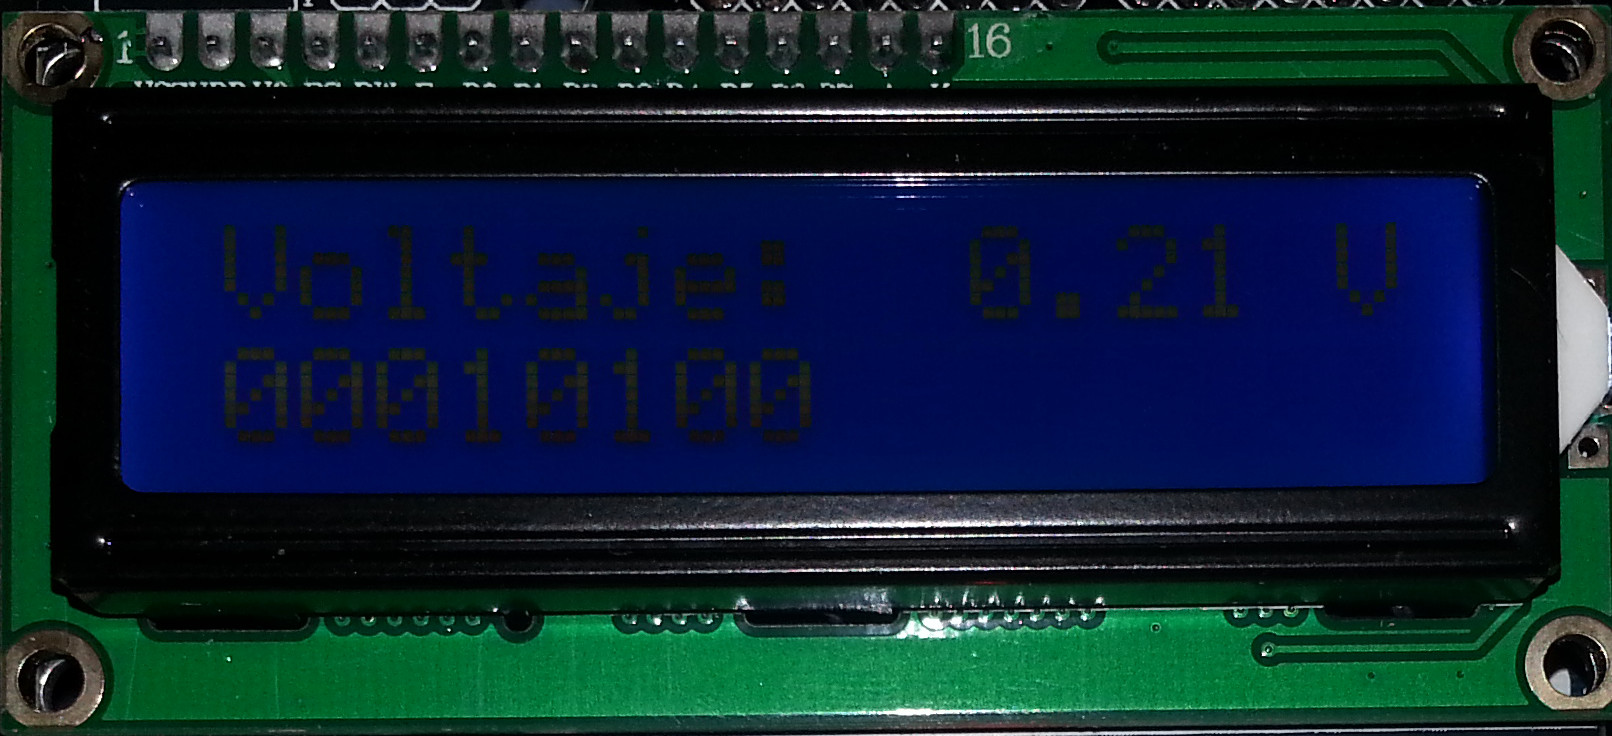
\includegraphics[scale=0.25]{images/lcd.jpg}\caption{Prueba LCD}
			\end{figure}

	\newpage
	\section{Referencias}
		\label{sec:referencias}

\end{document}
